\chapter{Sequential simulator}
\label{ch:sequential}

In other to begin the implementation of the simulator, a initial version was
considered with the minimum complexity, to verify the correctness of the model.
A graphic subsystem was build with MathGL and OpenGL to produce realtime plots
of different elements of the simulation. Of special interests are the particle
motion, the electric potential and the electric field.

The language of choice was C for the low overhead, the lack of automatic memory
management, the support of different libraries planned in future versions and
the low level design, which allowed us to define most of the data structures
close to the byte level.

\section{Design}

The simulator initially only supported one group of particles of the same charge
and mass, denominated specie. Each particle was implemented as a structure with
a given index $i$, a position vector $\x$, velocity $\v$ and other extra fields
such as the interpolated electric field at the particle position $\E$.
%
The fields were allocated in contiguous arrays, with the $x$ dimension aligned
with the cache line, also called row-major storage.

The configuration of the simulation is specified in plain configuration files,
with the syntax defined by the \texttt{libconfig} library. Is important to allow
the user to specify comments in the configuration files, as well as scientific
notation in different values. Additionally, the specification of multiple species
benefits from the sub-configuration block feature, which leads to a more
intuitive representation. The detailed configuration is described in the
chapter~\ref{ch:config}.

The solver used was initially the $LU$ decomposition, used from the $GSL$
numeric library~\cite{gsl}, as the only focus was to obtain valid results, ignoring the
performance. All implementations are tested beforehand with some test cases
designed in \texttt{octave}.

\section{Validation}

A set of different tests were designed to determine the correctness of the
simulation.

\subsection{Two particle test}

A simple test consists of two electrons placed at some distance different of
$L/2$ with no initial speed. The analytical solution is known and the motion 
should follow a harmonic oscillation trajectory. The energy conservation can be 
observed in the figure~\ref{fig:1d-2particles-energy}, where the total energy 
only varies due to the interpolation noise as the time $t$ grows in the $x$ 
axis.
%
\begin{figure}[h]
	\centering
	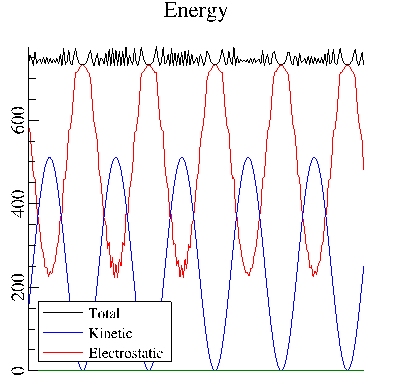
\includegraphics[width=0.4\linewidth]{1d-2particles-energy.png}
	\caption{Energy conservation in two particle test}
	\label{fig:1d-2particles-energy}
\end{figure}
